\section{Máquina Virtual (MV)}
\label{chp:referencial_teorico::sct:maquina_virtual}
Temos a MV e esta precisa do hypervisor. Como exemplo digamos que temos um dispositivo de armazenamento o qual interage diretamente com o hypervisor através de seus drivers, o hypervisor gera um driver virtual do qual é utilizado dentro da MV para interagir com o SO convidado \cite{docker_diff_standard_virt}.

O caso da máquina virtual, normalmente é utilizado visando rodar múltiplos SOs diferentes e até de arquiteturas diferentes. Como seu uso implica na utilização de um hypervisor, temos o isolamento dos recursos.

Possuindo em si algumas outras segmentações, tais como a virtualização de tipo 1 (bare-metal) e tipo 2. Como visualização das diferenças entre os tipos de virtualização providos por MVs, temos a figura \ref{fig:virtualization_t1_vs_t2} ilustrativa dos conceitos que serão falados logo a seguir \cite{kernelscheepers, Virtualization_vs_Containerization}.

\begin{figure}
    \centering
    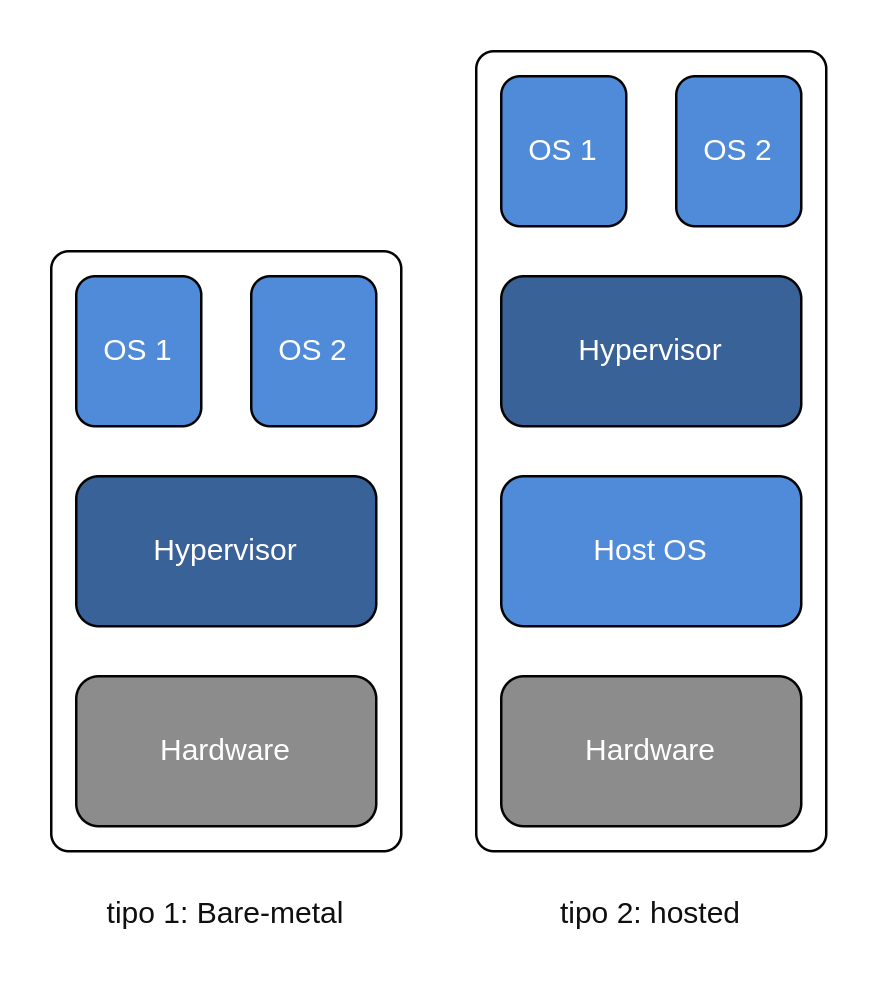
\includegraphics[width=8cm]{images/vm_t1_vs_t2.drawio.png}
    \caption{Virtualização tipo 1 vs tipo 2}
    \label{fig:virtualization_t1_vs_t2}
\end{figure}

\paragraph*{Tipo 1 - Bare-metal}\mbox{}\\
No tipo de virtualização bare-metal, temos o hypervisor que cuida de todo o gerenciamento do recurso e distribuição dos mesmos para cada SO convidado. Possuem performance melhor em comparação ao tipo 2, uma vez que seu acesso intercede exclusivamente o hypervisor, assim rodando praticamente de forma nativa, devido as camadas demonstrada na figura \ref{fig:virtualization_t1_vs_t2}.

A respeito deste tipo, o GNU/Linux implementa um módulo kernel-based virtualization machine (KVM), o qual resulta na capacidade de virtualização sobre este funcionar tal como um hypervisor. Deste modo, praticamente qualquer kernel Linux com este módulo pode ser utilizado tal como um hypervisor \cite{what-is-KVM}.

\paragraph*{Tipo 2 - Hosted Hypervisor}\mbox{}\\
Já no tipo 2, inicia-se um SO principal, e este através de virtualização de hardware e/ou tradução de interfaces binárias, possibilita o uso de recursos em um SO convidado. A comunicação do SO convidado com os recursos tende a ser mais demorada devido sua comunicação levar seu tempo de interpretação do SO principal, que por fim acessa o recurso solicitado, resultando assim em uma execução mais lenta quando comparado a virtualização tipo 1 bare-metal, conforme o aumento de camadas na figura \ref{fig:virtualization_t1_vs_t2}.
